% flashcards-title: A positive movement from negative one
% flashcards-desc: A signed number line arrow moves four units right from negative one to positive three.
\documentclass[dvisvgm,tikz,border=8pt]{standalone}
\usetikzlibrary{arrows.meta,patterns}

\definecolor{qraNavy}{HTML}{17324D}
\definecolor{qraBlue}{HTML}{2B6CB0}
\definecolor{qraGold}{HTML}{B7791F}
\definecolor{qraPale}{HTML}{EAF2F8}
\definecolor{qraGray}{HTML}{5C6773}

\tikzset{
  qra axis/.style={draw=qraNavy, line width=1.2pt},
  qra tick/.style={draw=qraNavy, line width=1pt},
  qra guide/.style={draw=qraGray, densely dashed, line width=0.8pt},
  qra counter/.style={circle, draw=qraNavy, fill=qraPale, line width=0.9pt, minimum size=7mm, inner sep=0pt},
  qra label/.style={font=\sffamily\bfseries, text=qraNavy},
  qra small label/.style={font=\sffamily, text=qraNavy},
}

\begin{document}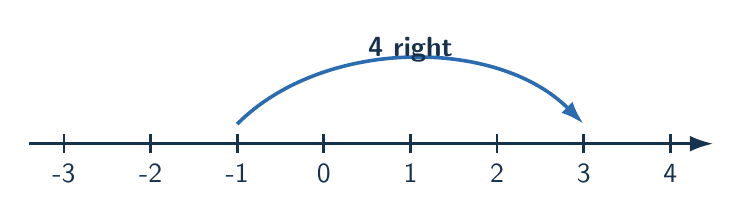
\begin{tikzpicture}[x=1.1cm,y=1cm]
\draw[qra axis,-{Latex[length=3mm,width=2mm]}](-3.4,0)--(4.5,0);
\foreach \x in {-3,...,4}{\draw[qra tick](\x,-.12)--(\x,.12);\node[qra small label,below=4pt]at(\x,0){\x};}
\draw[qraBlue,line width=1.3pt,-{Latex[length=3mm,width=2mm]}](-1,.25)..controls(0,1.35)and(2,1.35)..(3,.25);
\node[qra label]at(1,1.2){4 right};
\end{tikzpicture}\end{document}
